%%%%%%%%%%%%%%%%%%%%%%%%%%%%%%%%%%%%%%%%%
% Beamer Presentation
% LaTeX Template
% Version 1.0 (10/11/12)
%
% This template has been downloaded from:
% http://www.LaTeXTemplates.com
%
% License:
% CC BY-NC-SA 3.0 (http://creativecommons.org/licenses/by-nc-sa/3.0/)
%
%%%%%%%%%%%%%%%%%%%%%%%%%%%%%%%%%%%%%%%%%

%----------------------------------------------------------------------------------------
%	PACKAGES AND THEMES
%----------------------------------------------------------------------------------------

\documentclass{beamer}

\mode<presentation> {

% The Beamer class comes with a number of default slide themes
% which change the colors and layouts of slides. Below this is a list
% of all the themes, uncomment each in turn to see what they look like.

%\usetheme{default}
%\usetheme{AnnArbor}
%\usetheme{Antibes}
%\usetheme{Bergen}
%\usetheme{Berkeley}
%\usetheme{Berlin}
%\usetheme{Boadilla}
%\usetheme{CambridgeUS}
%\usetheme{Copenhagen}
%\usetheme{Darmstadt}
%\usetheme{Dresden}
%\usetheme{Frankfurt}
%\usetheme{Goettingen}
%\usetheme{Hannover}
%\usetheme{Ilmenau}
%\usetheme{JuanLesPins}
%\usetheme{Luebeck}
\usetheme{Madrid}
%\usetheme{Malmoe}
%\usetheme{Marburg}
%\usetheme{Montpellier}
%\usetheme{PaloAlto}
%\usetheme{Pittsburgh}
%\usetheme{Rochester}
%\usetheme{Singapore}
%\usetheme{Szeged}
%\usetheme{Warsaw}

% As well as themes, the Beamer class has a number of color themes
% for any slide theme. Uncomment each of these in turn to see how it
% changes the colors of your current slide theme.

%\usecolortheme{albatross}
%\usecolortheme{beaver}
%\usecolortheme{beetle}
%\usecolortheme{crane}
%\usecolortheme{dolphin}
%\usecolortheme{dove}
%\usecolortheme{fly}
%\usecolortheme{lily}
%\usecolortheme{orchid}
%\usecolortheme{rose}
%\usecolortheme{seagull}
%\usecolortheme{seahorse}
%\usecolortheme{whale}
%\usecolortheme{wolverine}

%\setbeamertemplate{footline} % To remove the footer line in all slides uncomment this line
%\setbeamertemplate{footline}[page number] % To replace the footer line in all slides with a simple slide count uncomment this line

%\setbeamertemplate{navigation symbols}{} % To remove the navigation symbols from the bottom of all slides uncomment this line
}

\usepackage{graphicx} % Allows including images
\usepackage{booktabs} % Allows the use of \toprule, \midrule and \bottomrule in tables

\usepackage{enumerate}   

\usepackage{float}
\setbeamertemplate{bibliography item}{\insertbiblabel}

%----------------------------------------------------------------------------------------
%	TITLE PAGE
%----------------------------------------------------------------------------------------

\title[An Elegant Grating coupler]{An Elegant Grating coupler for high resolution Beam Scanning} % The short title appears at the bottom of every slide, the full title is only on the title page

\author{Sanam Moslemi-Tabrizi} % Your name
\institute[] % Your institution as it will appear on the bottom of every slide, may be shorthand to save space
{
Carleton University \\ % Your institution for the title page
\medskip
\textit{smoslemi@yahoo.ca} % Your email address
}
\date{\today} % Date, can be changed to a custom date

\begin{document}

%\begin{frame}
%\titlepage % Print the title page as the first slide
%\end{frame}
%
%\begin{frame}
%\frametitle{Overview} % Table of contents slide, comment this block out to remove it
%\tableofcontents % Throughout your presentation, if you choose to use \section{} and \subsection{} commands, these will automatically be printed on this slide as an overview of your presentation
%\end{frame}
%
%%----------------------------------------------------------------------------------------
%%	PRESENTATION SLIDES
%%----------------------------------------------------------------------------------------
%
%%------------------------------------------------
%\section{GC basics} % Sections can be created in order to organize your presentation into discrete blocks, all sections and subsections are automatically printed in the table of contents as an overview of the talk
%\begin{frame}
%\frametitle{GC Basics}
%\begin{itemize}
%\item The basic grating coupler is a periodic structure of teeth and groove with a grating period of $d$ and the coupling angle of $\theta.$ 
%\item Because of the periodic structure there will be a leakage process from the waveguide which results in coupling out the light into the free space. 
%\item This leakage process highly depends on the physical structure of the waveguides and grating such as index of reflection of the materials($n_g$, $n_{cl}$, $N_{eff}$, $\dots$ ), the groove depth($t_g$), the pitch size($d$), length of grating ($L$) and the wavelength of the input light ($\lambda $) and even more.
%\item The leaky wave consist of an infinite space harmonic waves with a complex propagation of $k_n= \beta_n + i\alpha$ where $\alpha$ is the leakage factor and $\beta_n$ is the space harmonic propagation constant defined as below [2] and [3]:
%$\beta_n \, = \, \beta_0 \, + \, \frac{2n\pi}{d} \quad n=0 \, , \,  \pm1 \, , \, \pm2 \, , \, \dots$
%\item The radiation angle from the GC to the air is defined by $\sin(\theta_n)=\frac{\beta_n}{k_0}  \, = \,\frac{\beta_0 +\frac{2n\pi}{d}}{k_0} \quad n=0 \, , \,  \pm1 \, , \, \pm2 \, , \, \dots$
%
%\end{itemize}
%\end{frame}
%%
%\section{Design Constraints and Spec} 
%\begin{frame}
%\subsection{Effective index} 
%\frametitle{Effective index}
%\begin{itemize}
%\item  To have a valid radiation angel ($\theta_n$) we should have $|\frac{\beta_0 +\frac{2n\pi}{d}}{k_0}| <1$. We also know that $\beta_0 > k_0$. This conclude that n must be negative.
%\item Depending on the physical structure there will multiple outgoing beams, however in our application we wanted to have one strong outgoing beam so we design our GC for $n \, = \, -1$.  Taking into account our spec and following the physics explained in the referred papers  we must satisfy the following conditions
%\begin{eqnarray*}
%|\beta_0 -\frac{2\pi}{d}| <k_0 & => & |N_{eff}-\frac{\lambda}{d}| < 1\\
%|\beta_0 -2\frac{2\pi}{d}| >k_0 & => & |N_{eff}-2\frac{\lambda}{d}| > 1\\ \\
%|\beta_0 -2\frac{2\pi}{d}| >k_0 \sqrt{\epsilon_s} & => & |N_{eff}-\frac{\lambda}{d}| > \sqrt{\epsilon_s} \\
%N_{eff} & \neq & \frac{\lambda}{d} 
%\end{eqnarray*}
%\end{itemize}
%\end{frame}
%%
%\begin{frame}
%\frametitle{Effective index valid area}
%In Figure (\ref{neff1}) we showed the region for valid parameters to choose for forward or backward propagations
%\begin{figure}[H]
%\begin{center}
%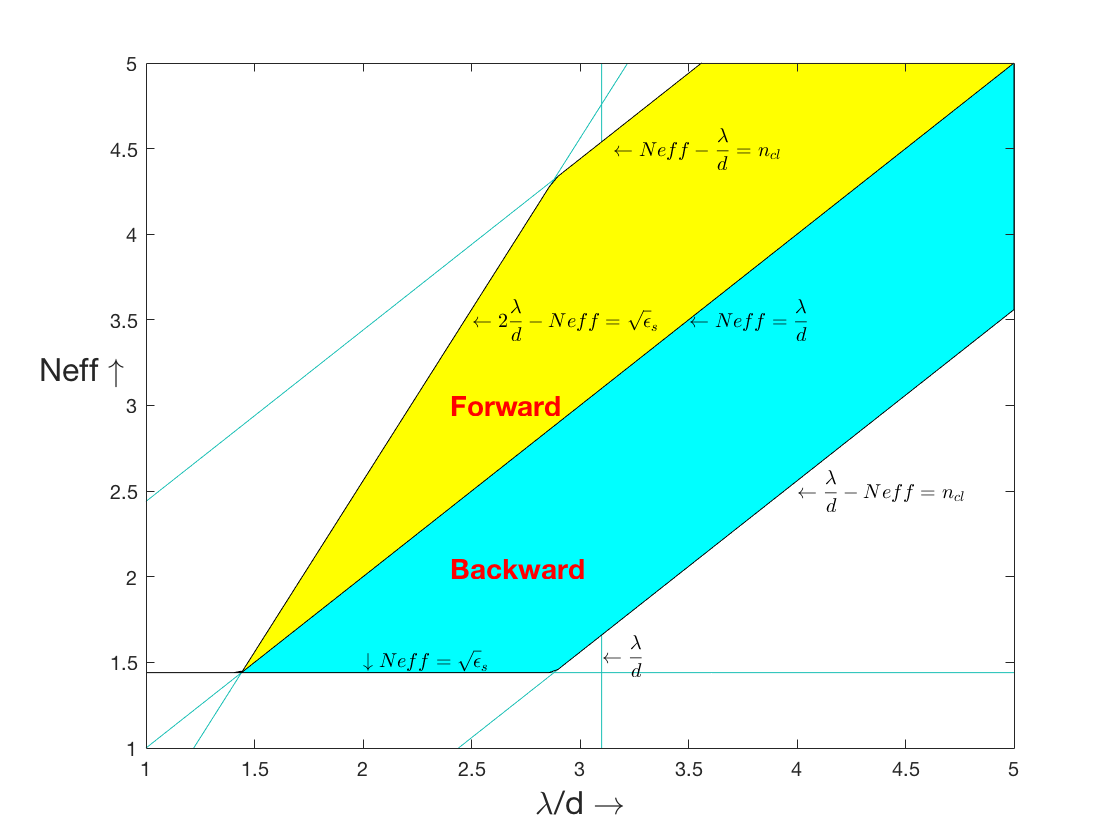
\includegraphics[width=10cm, height=7cm]{Figures/neffConstraint}
%\caption{Valid Regions for forward or backward propagations}
%\label{neff1}
%\end{center}
%\end{figure}
%\end{frame}
%%
%\subsection{Narrow beam} 
%\begin{frame}
%\frametitle{Narrow beam}
%\begin{itemize}
%\item Resolution scanning is defined by $FOV/\delta \lambda_{FWHM}$. So we need to be able to generate a very narrow beam to increase the resolution (lower $\delta \lambda_{FWHM}$).
%    \begin{equation}
%    \delta \lambda_{FWHM} \, = \, \frac{\lambda^2}{2 \pi L N_{g_c}}
%    \end{equation}
%\item To get a narrow beam we need to increase the length and/or increase the group index.
%\item Increasing the length will increase the transmission loss and also that will increase the size of the device. Also at some point of longitudinal length we will get to the saturation where increasing length won't be effective, because by the most of the light is already saturated.
%\item With group index, we have more room to engineer the desired material for us using SWG. 
%\end{itemize}
%\end{frame}
%%
%\begin{frame}
%\frametitle{Narrow beam (continued)}
%\begin{itemize}
%\item  The group index is highly depended on the physical features of the grating such as the pitch size, duty cycle and etching depth. Among those the etching depth is process depended variable and there are limitation on it. Non uniform Shallow etching will have a huge impact on $N_{g_c}$ and $\delta \lambda_{FWHM} $,  however fabrication for non uniform shallow etching is costly and difficult, therefore we are replacing the effect of etching depth by using sub wavelength grating on the materials to achieve the desired small FWHM. It is proven that using combination of Silicon and Sio2 we can engineer materials with effective index between 1.44 and 3.47 with changing the duty of cycle go SWG. 
%\begin{eqnarray*}
%n^2_	\parallel \,= \, f_{swg} n^2_1 \, + \, (1-f_{swg})n^2_2 \\
%1/n^2_\perp \,= \, f_{swg} /n^2_1 \, + \, (1-f_{swg})/n^2_2 
%\end{eqnarray*}
%\item For the GC the effective index is dependent on the duty cycle of grating (f) as $N_{g} = f n_g \, + \, (1-f)n_t$
%\end{itemize}
%\end{frame}
%%
%\subsection{Low loss}
%\begin{frame}
%\frametitle{Low loss}
%\begin{itemize}
%\item  The duty cycle of the grating and the difference in permittivity of the grating and top cladding effects the leakage factor of the grating. For a rectangular grating this dependency in described as below:
%    \begin{equation}
%    \alpha \simeq (\epsilon_r \,- \, \epsilon_{cl})^2 \, \sin^2(\pi f /d)
%    \end{equation}
%\item For minimum loss the index of grating and cladding should be as close as possible (again SWG will help us with that) and also we need to keep away from f=0.5 duty cycle. Again here need would need an \underline{optimization} for $f$.
%\item Thickness of grating ($t_g$) also affects the leakage. Increasing $t_g$ will increase the leakage but at some point we will get to the saturation point where leakage only have small oscillations as shown in figure \ref{loss1}.
%\end{itemize}
%\end{frame}
%%
%\begin{frame}
%\frametitle{Low loss (continued)}
%\begin{figure}[H]
%\begin{center}
%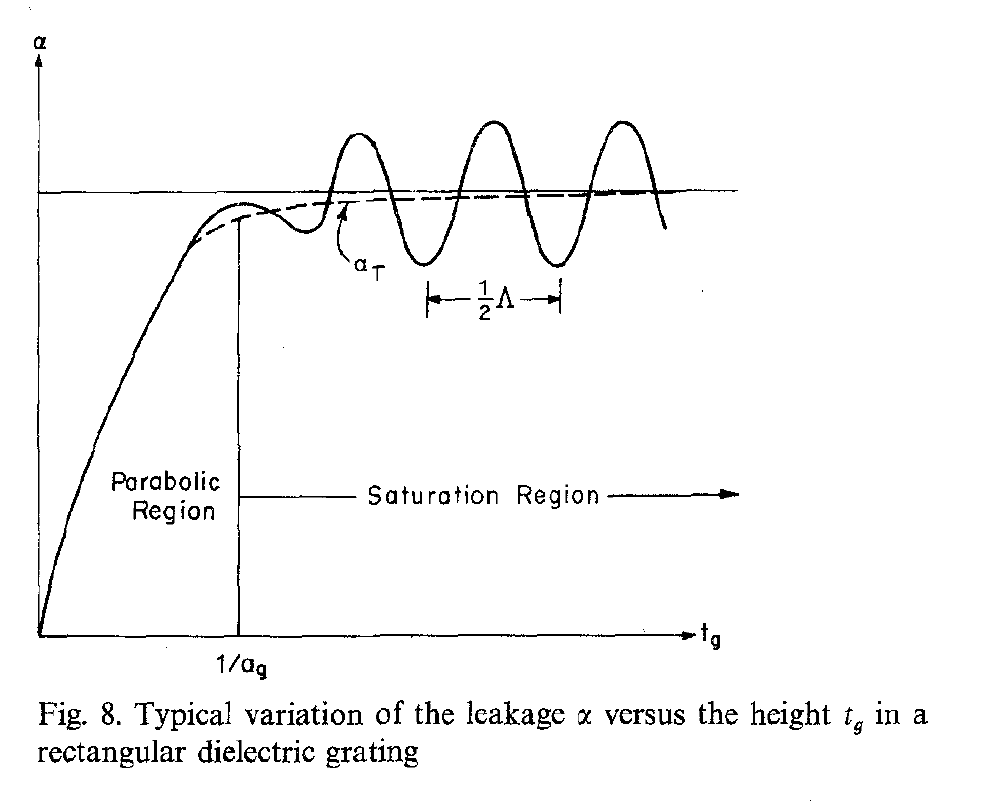
\includegraphics[width=10cm, height=7cm]{Figures/leakagevsthickness}
%\caption{leakagevsthickness}
%\label{loss1}
%\end{center}
%\end{figure}
%\end{frame}
%%
%\begin{frame}
%\subsection{Grating thickness}
%\frametitle{Low loss, grating thickness}
%\begin{itemize}
%\item  Following the perturbation analysis for the GC in reference [5] we  get to the following points:
%\begin{eqnarray*}
%\gamma_{q_{-1}} \, = \, k_0\sqrt{\epsilon_q \, - \, (N \, - \frac{\lambda}{d})^2 } \\
%\Lambda_{g_{-1}} = \frac{2\pi}{\gamma_{g_{-1}} } =  \frac{\lambda}{\sqrt{\epsilon_g \, - \, (N \, - \frac{\lambda}{d})^2}  } 
%\end{eqnarray*}
%    \begin{itemize}
%    \item $q$ identifies the layers (substrate, thin film, grating, cladding) (see figure \ref{gratingRegion1})
%    \item $\Lambda_{g_{-1}}$ is the oscillations period in the saturation region.
%    \item $t_{g_{cross over}} \, = \, \frac{\Lambda_{g_{-1}}}{4} $. 
%    	\begin{itemize}
%	\item $t_g \, < t_{g_{cross over}} $ is in Parabolic Region
%	\item $t_g \, > t_{g_{cross over}} $ is in Saturation Region
%	\end{itemize}
%    \end{itemize}
%\end{itemize}
%\end{frame}
%%
%\begin{frame}
%\frametitle{Low loss, grating thickness (continued)}
%\begin{figure}[H]
%\begin{center}
%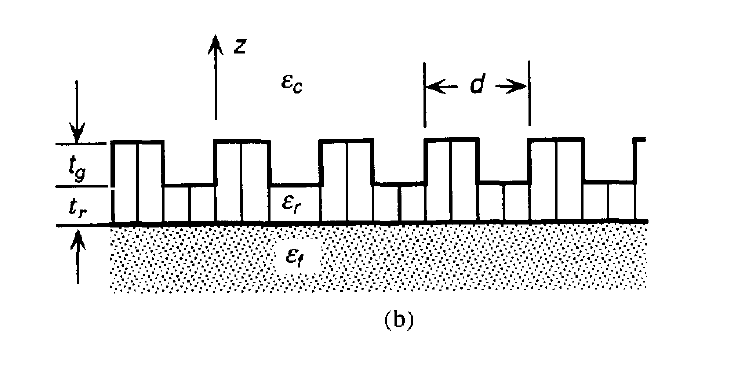
\includegraphics[width=5cm, height=4cm]{Figures/gratingStruc} 
%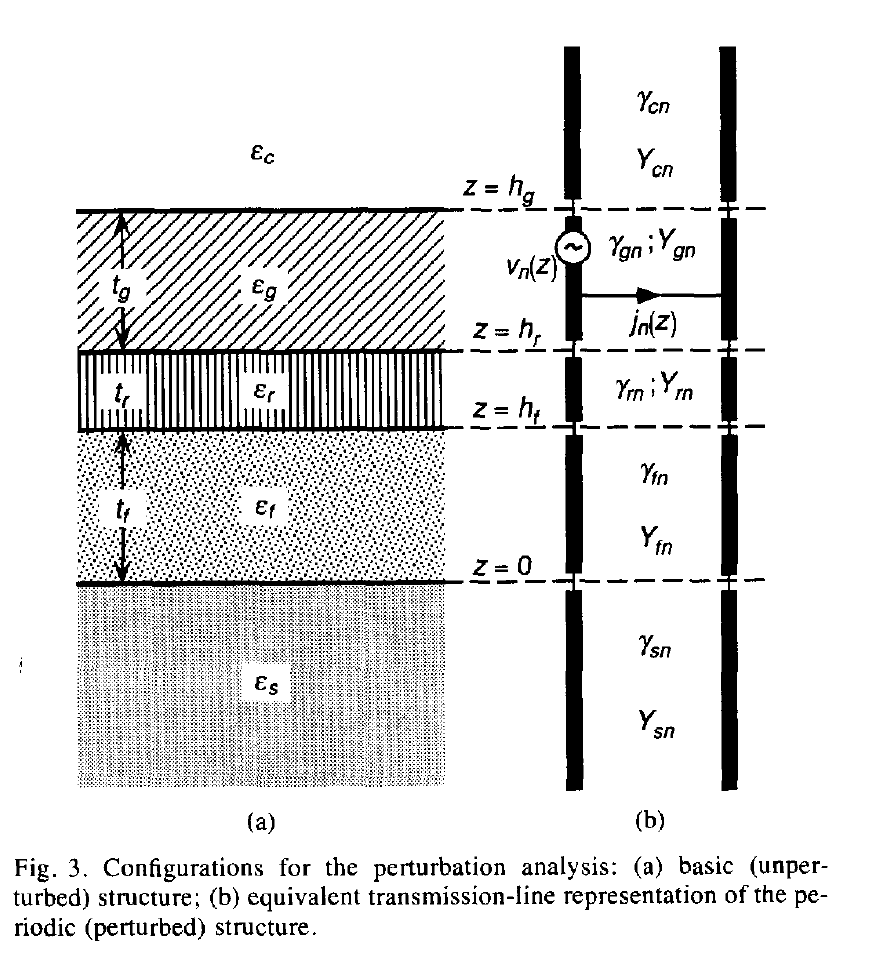
\includegraphics[width=8cm, height=6cm]{Figures/perturbationAnalysis}
%\caption{grating regions}
%\label{gratingRegion1}
%\end{center}
%\end{figure}
%\end{frame}
%%
%\section{Optimization} 
%\begin{frame}
%\frametitle{Optimization on GC}
%\begin{itemize}
%\item  The design of GC involves many parameters. Based on fundamental physics of GC we can define some of them but not all.
%\item We need to run iterations and then choose the best design. This process can be time consuming
%\item Using Principal Components Analysis we can reduce he dimension of our variables which will result in reduction of iteration which will save time.
%\end{itemize}
%\end{frame}
%%
%\section{Numerical results} 
%\begin{frame}
%\frametitle{Numerical results}
%\begin{itemize}
%\item  Here is the output of my design, it is a valid design but can be even more optimized. In the conference there was a talk on AI and PIC (from NRC Ottawa), which was really interesting. I'm going to apply the "Principal Components Analysis" on this GC design and see if I can get to better optimizes solution.
%\begin{figure}[H]
%%\begin{center}
%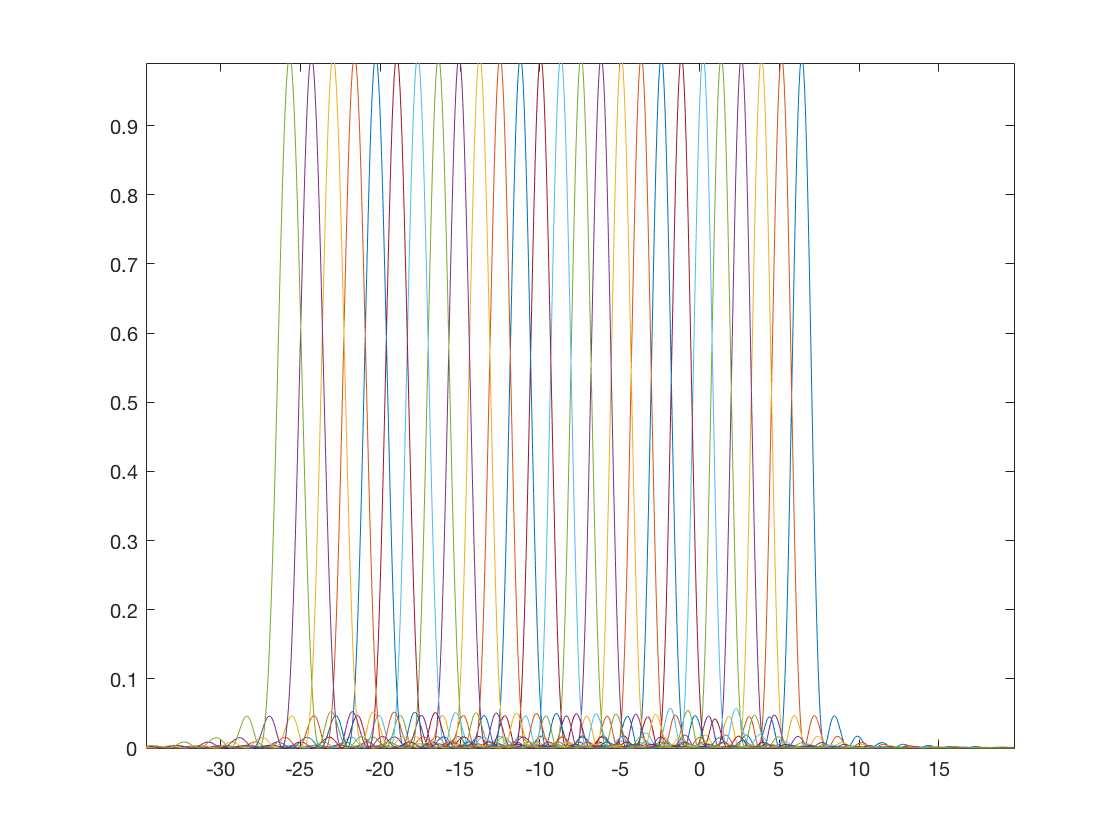
\includegraphics[width=8cm, height=6cm]{Figures/fov1335_1360}
%\caption{Desgined GC}
%\label{numerical results}
%%\end{center}
%\end{figure}
%\end{itemize}
%\end{frame}
%%
%\begin{frame}
%\frametitle{Numerical results}
%\begin{itemize}
%\item  Using this structure I could achieve a narrow beam with $FWHM \, = \, 1^{\circ}$ and a $FOV \,  = \, 32^{\circ}$, which gives us a resolution of 32. This is higher resolution than what is in the literature.
%\item Based on [6]"To date, OPA steering resolution has been limited. To our knowledge, the widest demonstrated steering range of any OPA
%was $51^{\circ}$; however, the beam divergence was relatively large $(3.3^{\circ})[9]$. The narrowest beam divergence was $0.3^{\circ}$; however, the steerable range was relatively small $(0.9^{\circ}) [12]$. The highest-resolution device had a resolution of 23, achieving the best ratio of steering range to beam divergence $(23^{\circ}$ and $1^{\circ}$, respectively) [10]."
%\end{itemize}
%\end{frame}
%%
%\section{Phase Shifting} 
%\begin{frame}
%\frametitle{Phase Shifting}
%\begin{itemize}
%\item  At the conference there were talks about PIN depletion based phase shifting (the phase shifting were more for modulation and not beam scanning)
%\item One researcher actually described the fabrication process for their PIN design. It tells me that we were on the right thought with the idea in our very preliminary design. 
%\item In general there were designs that looked fabrication challenging but there was not much emphasis on that. Fabrication processes in improving as we go.
%\end{itemize}
%\end{frame}
%%
%\section{Mode Analytics} 
%\begin{frame}
%\frametitle{Mode Analytics}
%Design spec for waveguide:
%\begin{enumerate}
%\item Fundamental mode must be TE.\label{spec1}
%\item To be single mode over the range of wavelength sweep. \label{spec2}
%\item Because of Silicon transparency window, the wavelength must be over $1.1 \mu m$
%\item Because of the fabrication limitations the hight is $b=220 nm$.
%\end{enumerate}
%%
%\begin{itemize}
%\item  For a rectangle waveguide $a \times b$ where a is the width and b is the hight we will have a cut off frequency defined by
%\begin{equation}
%f_c =\frac{c}{2\pi N} \sqrt{(\frac{m\pi}{a})^2 +(\frac{n\pi}{b})^2}
%\end{equation}
%$f_c$ is the lowest frequency (the largest wavelength) generating propagation in the waveguide which is dictated by the dimensions of the waveguide and it's material (index of refraction). 
%\end{itemize}
%\end{frame}
%%
%\begin{frame}
%\frametitle{Mode Analytics Continued}
%\begin{itemize}
%\item To fulfill specs \ref{spec1}-\ref{spec2} the first two modes must be $m=0$ or $n=0$ which would give us $TE_{10}$ and $TE_{01}$. Frequencies associated with these 2 mode with define the the input laser wavelength window.
%\item I put these constraints and specs  in a Matlab code and generate the possible design options. 
%\item Going through the option we see that with a width of 300 or 400 nm, with the index of refraction between 2.7 to 2.9 we can satisfy our design spec.
%\item Lumerical's Mode Solution also confirmed the Matlab data.
%\end{itemize}
%\end{frame}
%%
%\section{swg; fundamentals} 
%\begin{frame}
%\frametitle{Horizontal swg structure, swg strips are in parallel to direction of propagation }
%\begin{figure}[H]
%%\begin{center}
%\includegraphics[width=2cm, height=2cm]{Figures/swg_v}
%\includegraphics[width=5cm, height=5cm]{Figures/neff_Pitchswg0p1_W0p4_h0p22_Lswg_DCswg}
%\includegraphics[width=5cm, height=5cm]{Figures/neff_Pitchswg0p1_W0p4_h0p22_DCswg_Lswg}
%\caption{\small{Horizontal swg (swg strips are in parallel to direction of propagation), Length of grating ($L_{swg}$)the the length of the structure in the direction of propagation (x)}, simulation show that propagation starts at $L_swg \, >= \,0.7 \mu m$}
%\label{vSwg}
%%\end{center}
%\end{figure}
%
%\end{frame}
%%
\section{Mode; fundamentals} 
\begin{frame}
\frametitle{Meeting with Dusan}
 We had a meeting with Dusan (Myself, Dusan and Tom). I mentioned  Winnine and Tom's concerns about the FDE simulation region and the whole structure  and he  confirmed that the structure and the simulation size were valid (as I expected :-) )
\begin{itemize}
\item He suggested that I can increase the width of the sio2, not because the current structure is not valid, but because in real fabricated chips sio2 will be wider. 
\item He ran the structure with wider sio2 in a way that FDE region was inside the sio2 (based on the structure I was given on our skye call) and the result didn't change much (as expected).
\item About an extra layer of Substrate of Si underneath of sio2, Dusan mentioned if my sio2 is thick enough I won't need it (as expected).
\end{itemize}
So based on yesterday's meeting the structure was valid and so would be the simulation results. So I will carry on with my plan as follows.
\end{frame}
%\section{Mode; fundamentals} 
%\begin{frame}
%\frametitle{Structure Under Test}
%This is our structure under test. I first built it in Mode Solution.
%\begin{figure}[H]
%%\begin{center}
%\includegraphics[width=10cm, height=6cm]{Figures/modes/wg_mode_mod}
%\end{figure}
%\end{frame}
%%
%\begin{frame}
%\frametitle{Structure Under Test (continued)}
%Next I used the exact same structure in FDTD Solution.
%\begin{figure}[H]
%%\begin{center}
%\includegraphics[width=10cm, height=6cm]{Figures/modes/wg_fdtd}
%\end{figure}
%\end{frame}
%%
%\begin{frame}
%\frametitle{Mode Analysis (continued)}
%I run 3 types of simulation to find $n_{eff}$ on this structure.
%\begin{itemize}
%\item Mode Solution (which is a 2D simulation)
%\item Mode expansion in FDTD Solution (which is also 2d and very similar to the Mode Solution tool).
%\item 3D FDTD and calculate/measure the $n_{eff}$ from the E field data. ($\lambda_n = \lambda_0/n_{eff})$
%\end{itemize}
%I basically changed Material index in the range of 3.476 - 1.75 and run the solvers. \\
%In Mode solution I run the simulation and capture the mode index for each material index. \\
%In FDTD in used 2 types of monitors, Field Monitor and Mode Expansion Monitor.
%\end{frame}
%%
%\begin{frame}
%\frametitle{Mode Analysis (continued)}
%\begin{itemize}
%\item in Field monitor, I measured and calculated $n_{eff}$ as we discussed last week (measuring the peaks to find $\lambda_n$ and then $n_{eff}= \lambda_0 /\lambda_n$.  I also start working on $\eta = E/H  \;  \Longrightarrow \; \epsilon_n \;  \Longrightarrow \; n_{eff}$ but it is not done yet.
%\item Mode expansion monitor in FDTD solution is very similar to Mode tool, it just directly calculates the $n_{eff}$ but in 2D only.
%\end{itemize}
%\end{frame}
%%
%\begin{frame}
%\frametitle{Numerical results}
%\begin{figure}[H]
%This is a graph of Mode index vs Material index of the under test waveguide with fixed width of  0.5 $\mu m$
%\includegraphics[width=10cm, height=6cm]{/Users/sanam/phd/lidarGit/lidar/docs/presentation/gc/Data/ModeIndex_vs_MaterialIndex_fixedWidth.png}
%\end{figure}
%\end{frame}
%%
%\begin{frame}
%\frametitle{Numerical results (continued)}
%Example Mode Profiles obtained from Mode Solution \\
%Material index of the wg = 3.25 \\
%resulted mode index = 2.12789
%\begin{figure}[H]
%\includegraphics[width=10cm, height=6cm]{Figures/modes/mode1_effMaterial1}
%\end{figure}
%\end{frame}
%%
%\begin{frame}
%\frametitle{Numerical results (continued)}
%Example Mode Profiles obtained from Mode Solution \\
%Material index of the wg = 3.0 \\
%resulted mode index = 1.85445
%\begin{figure}[H]
%\includegraphics[width=10cm, height=6cm]{Figures/modes/mode1_effMaterial2}
%\end{figure}
%\end{frame}
%%
%\begin{frame}
%\frametitle{Numerical results (continued)}
%Example Mode Profiles obtained from Mode Solution \\
%Material index of the wg = 2.5\\
%resulted mode index = 1.41981
%\begin{figure}[H]
%\includegraphics[width=10cm, height=6cm]{Figures/modes/mode1_effMaterial4}
%\end{figure}
%\end{frame}
%%
%\begin{frame}
%\frametitle{Numerical results (continued)}
%And to the point where there is no more propagation in the waveguide
%Material index of the wg = 2.0 \\
%resulted mode index = 1.32151
%\begin{figure}[H]
%\includegraphics[width=10cm, height=6cm]{Figures/modes/mode1_effMaterial6}
%\end{figure}
%\end{frame}

\begin{frame}
\frametitle{Next steps}
\begin{enumerate}%[(a)]
\item So far I run the simulations with a fixed width, \underline{next I'll sweep width and do the previous procedure for each width}. Previous procedure was to capture $n_{eff}$ from 3 sources of simulation and plot Mode index vs Material index. And the 3 simulation sources are Mode Solution sims, 3D FDTD sim and Modex expansion monitor in FDTD. This is the graph from the previous set of simulations.
\label{next1}
\begin{figure}[H]
\includegraphics[width=10cm, height=5cm]{/Users/sanam/phd/lidarGit/lidar/docs/presentation/gc/Data/ModeIndex_vs_MaterialIndex_fixedWidth.png}
\end{figure}
\end{enumerate}
\end{frame}

\begin{frame}
\frametitle{Next steps}
\begin{enumerate}
\setcounter{enumi}{1}
\item Based on the results of step (\ref{next1}) I'll choose a fixed width for our design with your confirmation and then will move to characterizing swg structures with that fixed width.
\begin{enumerate}[(a)]
\item 3D fdfd simuitation on a  swg vertical to find mode index vs swg duty cycle.
\item 3D fdfd simuitation on a  swg horizontal to find mode index vs swg duty cycle. 
\item Mod Solution simulation on the same swg horizontal to find mode index vs swg duty cycle. This is not valid for swg vertical.
\end{enumerate}
\item Find the graphs for Material Index vs Mode index vs duty cycle. This would be the fundamentals we need to know before we go to GC design.
\item Next would be to go back to my semi analytical GC design method using swg structures and finalize the design.
\end{enumerate}
\end{frame}
%
%\begin{frame}
%\frametitle{Next steps (continued}
%I also run one simulation with wider sio2 width, the index changes but not much. I'll run more examples to check.
%\begin{table}[htdp]
%\caption{Effect of sio2 width on Mode index}
%\begin{center}
%\begin{tabular}{|c|c|c|c|}
%\hline
%waveguide material & waveguide width & sio2 width & $n_{eff}$ \\
%\hline
%Silicon & 0.5 $\mu m$ & 1$\mu m$ &2.38542\\
%\hline
%Silicon & 0.5 $\mu m$ & 2 $\mu m$ &2.386392\\
%\hline
%\end{tabular}
%\end{center}
%\label{default}
%\end{table}%
%\end{frame}




%\begin{frame}
%\frametitle{Basics (cont.)}
%\begin{columns}[c] % The "c" option specifies centred vertical alignment while the "t" option is used for top vertical alignment
%
%\column{.55\textwidth} % Left column and width
%    \begin{figure}[htbp]
%    \begin{center}
%    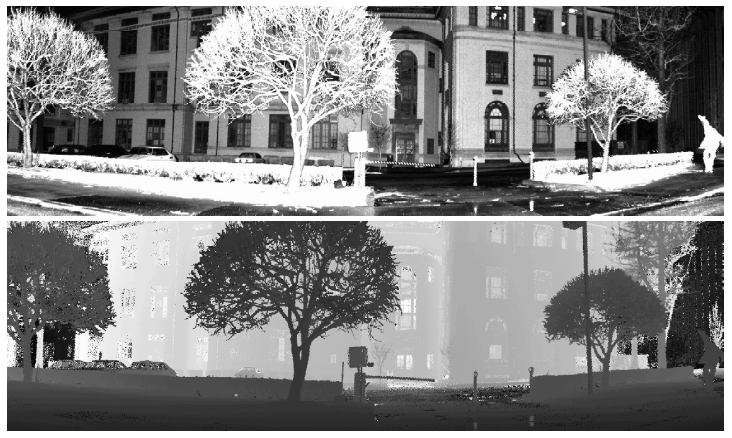
\includegraphics[width=6cm]{graphs/lidar_data}
%    \caption{LiDAR data}
%    \label{default}
%    \end{center}
%    \end{figure}
%
%\column{.5\textwidth} % Right column and width
%    \begin{figure}[htbp]
%    \begin{center}
%    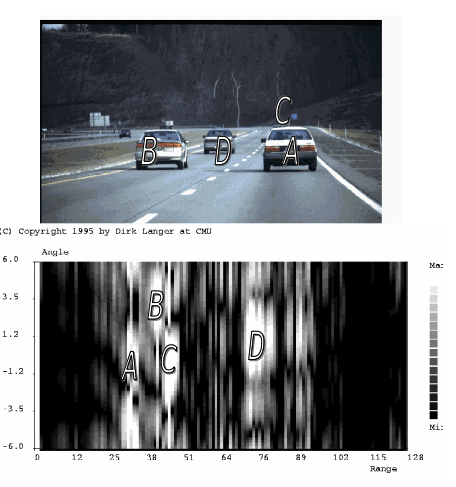
\includegraphics[width=6cm]{graphs/radar_data}
%    \caption{RADAR data}
%    \label{default}
%    \end{center}
%    \end{figure}
%
%\end{columns}
%\end{frame}
%
%%\begin{itemize}
%%\item Using proper modulation technique, it is possible the distance and velocity simultaneously \cite{pic0}.
%%\item Beam steering in the key element of LiDAR systems.
%%\end{itemize}
%
%\begin{frame}
%\frametitle{Basics}
%\begin{columns}[c] % The "c" option specifies centered vertical alignment while the "t" option is used for top vertical alignment
%
%\column{.55\textwidth} % Left column and width
%\begin{itemize}
%\item Tunable laser
%\item Semiconductor optical amplifiers 
%\item Splitters. MMI or Star coupler.
%\item Thermo-optical phase modulators (mainly resistive thermo optic phase shifters)
%\end{itemize}
%
%\column{.5\textwidth} % Right column and width
%   \begin{figure}[htbp]
%    \begin{center}
%    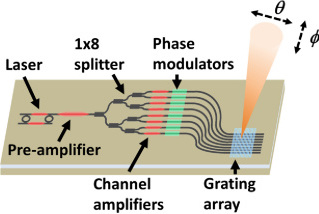
\includegraphics[width=6cm]{graphs/pic3}
%    \caption{An example LiDAR system \cite{pic3}}
%    \label{default}
%    \end{center}
%    \end{figure}
%
%\end{columns}
%\end{frame}
%%
%\begin{frame}
%\frametitle{Basics (cont.)}
%\begin{columns}[c] % The "c" option specifies centered vertical alignment while the "t" option is used for top vertical alignment
%
%\column{.55\textwidth} % Left column and width
%\begin{itemize}
%\item Channels and spacing
%    \begin{itemize}
%    \item The angular separation between the main lobe and the side lobes ($\phi$) is defined by spacing d: d$\searrow \;  \; \Rightarrow \;  \; \phi \; \nearrow$
%    \item The peak power of the side lobes is also a function of the ratio output waveguide width to channel d$\searrow \;  \; \Rightarrow \;  \;$ peak power  $\nearrow$
%    \item Very small spacing will cause crosstalk between channels
%    \item Non-uniform spacing \cite{pic2}
%    \end{itemize}
%\item Surface grating (pitch of 0.55 $\mu m$ nd a duty of 20$\%$)
%\end{itemize}
%
%\column{.45\textwidth} % Right column and width
%\begin{figure}[htbp]
%    \begin{center}
%    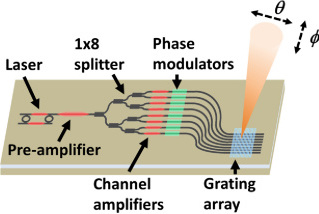
\includegraphics[width=5cm]{graphs/pic3}
%    \caption{An example LiDAR system \cite{pic3}}
%    \label{default}
%    \end{center}
%    \end{figure}
%
%\end{columns}
%\end{frame}
%
%%
%\section{Beam steering} 
%\begin{frame}
%\frametitle{Beam steering}
%\begin{itemize}
%\item By tuning wavelength, the beam in the far field can be steered in one axis ($\theta$)
%    \begin{equation}
%    \sin(\theta)\, =\, \frac{\Lambda n_{eff} - \lambda}{\Lambda }
%    \end{equation}
%\item The relative phase across the grating array determines the beam shape/direction in the other axis ($\phi$)
%\end{itemize}
%
%\begin{figure}[htbp]
%    \begin{center}
%    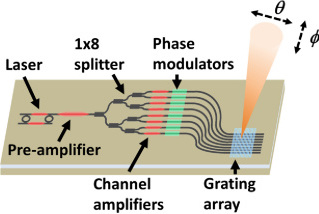
\includegraphics[width=8cm]{graphs/pic3}
%%    \caption{An example LiDAR system \cite{pic3}}
%    \label{default}
%    \end{center}
%    \end{figure}
% \end{frame}
%%
%\section{Examples} 
%\begin{frame}
%\frametitle{Another example}
%    \begin{figure}[htbp]
%    \begin{center}
%    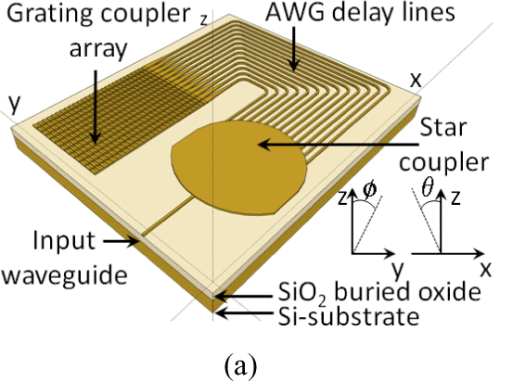
\includegraphics[width=6cm]{graphs/pic6_6}
%    \caption{An example LiDAR system \cite{pic6_opa}}
%    \label{default}
%    \end{center}
%    \end{figure}
%\end{frame}
%\begin{frame}
%    \begin{figure}[htbp]
%    \begin{center}
%    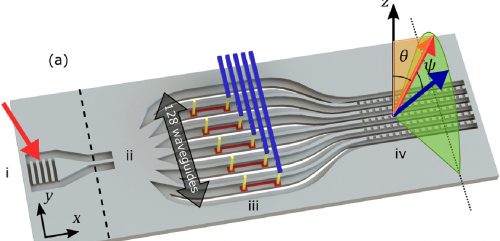
\includegraphics[width=8cm]{graphs/pic2}
%    \caption{An example LiDAR system \cite{pic2}}
%    \label{default}
%    \end{center}
%    \end{figure}
%\end{frame}
%\begin{frame}
%\frametitle{Another example}
%    \begin{figure}[htbp]
%    \begin{center}
%    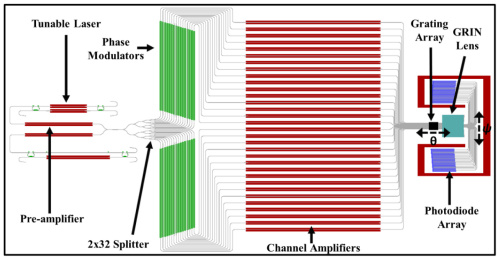
\includegraphics[width=10cm]{graphs/pic4}
%    \caption{An example LiDAR system \cite{pic4}}
%    \label{default}
%    \end{center}
%    \end{figure}
%\end{frame}
%%
%\begin{frame}
%\frametitle{MIT example}
%\begin{columns}[c] % The "c" option specifies centered vertical alignment while the "t" option is used for top vertical alignment
%
%\column{.7\textwidth} % Left column and width
%\begin{itemize}
%\item A LiDAR instrument with silicon photonic optical phased arrays.
%\item FMCW LIDAR allows for simultaneous Doppler-based velocity measurements.
%\item Triangular modulation is used to help with distance/velocity measurements.
%\item The time delay between RX and LO will create an electrical beat frequency.
%\item For a stationary target, this frequency is proportional to the distance of the target
%\item For a moving target, because of the Doppler shift on RX we will get two beat frequencies
%\item The difference of the two frequencies is twice the induced Doppler shift which is proportional to target's velocity.
%\end{itemize}
%\column{.4\textwidth} % Right column and width
%   \begin{figure}[htbp]
%    \begin{center}
%    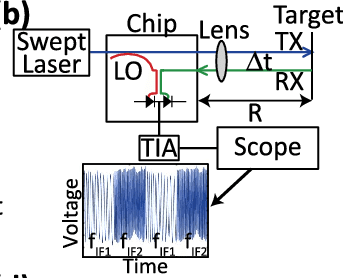
\includegraphics[width=4cm]{graphs/pic0}
%    \caption{\cite{pic0}}
%    \label{default}
%    \end{center}
%    \end{figure}
%
%\end{columns}
%
%\end{frame}
%
%
%
%%------------------------------------------------
%
%%\subsection{FMCW LIDAR with Triangular Modulation} % A subsection can be created just before a set of slides with a common theme to further break down your presentation into chunks
%
%%\begin{frame}
%%\frametitle{FMCW LiDAR}
%%\begin{itemize}
%%\itemThis system was fabricated within a 300 mm wafer CMOS compatible platform (low cost, can be integrated with CMOS Electronics). 
%%\item Integrated optical phased arrays with solid-state beam steering.
%%\item LiDAR than detect smaller objects with high resolution.
%%\item Using proper modulation technique, it is possible the distance and velocity simultaneously \cite{pic0}.
%%\item Beam steering in the key element of LiDAR systems.
%%\end{itemize}
%%\end{frame}
%
%%\begin{frame}
%%\frametitle{Paragraphs of Text}
%%Sed iaculis dapibus gravida. Morbi sed tortor erat, nec interdum arcu. Sed id lorem lectus. Quisque viverra augue id sem ornare non aliquam nibh tristique. Aenean in ligula nisl. Nulla sed tellus ipsum. Donec vestibulum ligula non lorem vulputate fermentum accumsan neque mollis.\\~\\
%%
%%Sed diam enim, sagittis nec condimentum sit amet, ullamcorper sit amet libero. Aliquam vel dui orci, a porta odio. Nullam id suscipit ipsum. Aenean lobortis commodo sem, ut commodo leo gravida vitae. Pellentesque vehicula ante iaculis arcu pretium rutrum eget sit amet purus. Integer ornare nulla quis neque ultrices lobortis. Vestibulum ultrices tincidunt libero, quis commodo erat ullamcorper id.
%%\end{frame}
%%
%%%------------------------------------------------
%%
%%\begin{frame}
%%\frametitle{Bullet Points}
%%\begin{itemize}
%%\item Lorem ipsum dolor sit amet, consectetur adipiscing elit
%%\item Aliquam blandit faucibus nisi, sit amet dapibus enim tempus eu
%%\item Nulla commodo, erat quis gravida posuere, elit lacus lobortis est, quis porttitor odio mauris at libero
%%\item Nam cursus est eget velit posuere pellentesque
%%\item Vestibulum faucibus velit a augue condimentum quis convallis nulla gravida
%%\end{itemize}
%%\end{frame}
%%
%%%------------------------------------------------
%%
%%\begin{frame}
%%\frametitle{Blocks of Highlighted Text}
%%\begin{block}{Block 1}
%%Lorem ipsum dolor sit amet, consectetur adipiscing elit. Integer lectus nisl, ultricies in feugiat rutrum, porttitor sit amet augue. Aliquam ut tortor mauris. Sed volutpat ante purus, quis accumsan dolor.
%%\end{block}
%%
%%\begin{block}{Block 2}
%%Pellentesque sed tellus purus. Class aptent taciti sociosqu ad litora torquent per conubia nostra, per inceptos himenaeos. Vestibulum quis magna at risus dictum tempor eu vitae velit.
%%\end{block}
%%
%%\begin{block}{Block 3}
%%Suspendisse tincidunt sagittis gravida. Curabitur condimentum, enim sed venenatis rutrum, ipsum neque consectetur orci, sed blandit justo nisi ac lacus.
%%\end{block}
%%\end{frame}
%%
%%%------------------------------------------------
%%
%%\begin{frame}
%%\frametitle{Multiple Columns}
%%\begin{columns}[c] % The "c" option specifies centered vertical alignment while the "t" option is used for top vertical alignment
%%
%%\column{.45\textwidth} % Left column and width
%%\textbf{Heading}
%%\begin{enumerate}
%%\item Statement
%%\item Explanation
%%\item Example
%%\end{enumerate}
%%
%%\column{.5\textwidth} % Right column and width
%%Lorem ipsum dolor sit amet, consectetur adipiscing elit. Integer lectus nisl, ultricies in feugiat rutrum, porttitor sit amet augue. Aliquam ut tortor mauris. Sed volutpat ante purus, quis accumsan dolor.
%%
%%\end{columns}
%%\end{frame}
%%
%%%------------------------------------------------
%%\section{Second Section}
%%%------------------------------------------------
%%
%%\begin{frame}
%%\frametitle{Table}
%%\begin{table}
%%\begin{tabular}{l l l}
%%\toprule
%%\textbf{Treatments} & \textbf{Response 1} & \textbf{Response 2}\\
%%\midrule
%%Treatment 1 & 0.0003262 & 0.562 \\
%%Treatment 2 & 0.0015681 & 0.910 \\
%%Treatment 3 & 0.0009271 & 0.296 \\
%%\bottomrule
%%\end{tabular}
%%\caption{Table caption}
%%\end{table}
%%\end{frame}
%%
%%%------------------------------------------------
%%
%%\begin{frame}
%%\frametitle{Theorem}
%%\begin{theorem}[Mass--energy equivalence]
%%$E = mc^2$
%%\end{theorem}
%%\end{frame}
%%
%%%------------------------------------------------
%%
%%\begin{frame}[fragile] % Need to use the fragile option when verbatim is used in the slide
%%\frametitle{Verbatim}
%%\begin{example}[Theorem Slide Code]
%%\begin{verbatim}
%%\begin{frame}
%%\frametitle{Theorem}
%%\begin{theorem}[Mass--energy equivalence]
%%$E = mc^2$
%%\end{theorem}
%%\end{frame}\end{verbatim}
%%\end{example}
%%\end{frame}
%%
%%%------------------------------------------------
%%
%%\begin{frame}
%%\frametitle{Figure}
%%Uncomment the code on this slide to include your own image from the same directory as the template .TeX file.
%%%\begin{figure}
%%%\includegraphics[width=0.8\linewidth]{test}
%%%\end{figure}
%%\end{frame}
%%
%%%------------------------------------------------
%%
%%\begin{frame}[fragile] % Need to use the fragile option when verbatim is used in the slide
%%\frametitle{Citation}
%%An example of the \verb|\cite| command to cite within the presentation:\\~
%%
%%This statement requires citation \cite{p1}.
%%\end{frame}
%%
%%%------------------------------------------------
%%
%\begin{frame}
%\frametitle{References}
%\footnotesize{
%\begin{thebibliography}{99} % Beamer does not support BibTeX so references must be inserted manually as below
%\bibitem1- [Dirk TAILLAERT and Frederik VAN LAERE, 2006]{pub2000} Dirk TAILLAERT and Frederik VAN LAERE, The Japan Society of Applied Physics (2006)
%\newblock Grating Couplers for Coupling between Optical Fibers and Nanophotonic Waveguides
%%
%% oe241821027beamwidth
%\bibitem 2- [FAEZEH FESHARAKI and NADIR HOSSAIN, 2016]{} FAEZEH FESHARAKI and NADIR HOSSAIN, Optics Express (2016)
%\newblock Accurate theoretical and experimental characterization of optical grating coupler
%%
%% tamirPeng1977
%\bibitem 3- [T Tamir and T. Peng, 1977]{} T Tamir and T. Peng,  Sensors(1977)
%\newblock Analysis and Design of Grating Couples
%%
%% hongChoSungFWHMsize
%\bibitem 4- [Yoo-Seung Hong and Chun-Hyung Cho, 2018]{} Yoo-Seung Hong and Chun-Hyung Cho,  Applied Physics by Spring Verlag(2018)
%\newblock Design Parameter Optimization of a Silicon-Based Grating Waveguide for Performance Improvement in Biochemical Sensor Application
%%
%% 00248941
%\bibitem 5- [Zhang and Tamir, 1993]{} Zhang and Tamir,  IEEE (1993)
%\newblock Analysis and Design of Broadband Grating couplers
%%
%% pic2
%\bibitem 6- [DAVID N. HUTCHISON and JIE SUN, 2016]{} DAVID N. HUTCHISON and JIE SUN,  IEEE (2016)
%\newblock High-resolution aliasing-free optical beam steering
%%
%%%\newblock \emph{Journal Name} 12(3), 45 -- 678.
%%%
%%\bibitem[J. K. Doylend, 2013]{pic3} J. C. Hulme, J. K. Doylend, M. J. R. Heck, J. D. Peters, M. L. Davenport, J. T. Bovington, L. A. Coldren, and J. E. Bowers(2013)
%%\newblock Hybrid silicon free-space source with integrated beam steering
%%%\newblock \emph{Journal Name} 12(3), 45 -- 678.
%%%
%%\bibitem[Christopher V.  Poulton,2017]{pic0} Christopher V.  Poulton, Ami Yaacobi,  Davis B. Cole, Mathew J. Byrd,  Manan Raval, Dierdrik Vermeulen,  and Michael R. Watts (2017)
%%\newblock Coherent solid-state LIDAR with silicon photonic optical phased arrays
%%%\newblock \emph{Journal Name} 12(3), 45 -- 678.
%%%
%%\bibitem[Wim Bogaerts, 2011]{pic6_opa} Karel Van Acoleyen, Wim Bogaerts, and Roel Baets, (2011)
%%\newblock Two-Dimensional Dispersive Off-Chip Beam Scanner Fabricated on Silicon-On-Insulator
%%%\newblock \emph{Journal Name} 12(3), 45 -- 678.
%%%
%%\bibitem[David N. Hutchison, 2016]{pic2} David N. Hutchison, Jie Sun, Jonathan K. Doylend, Ranjeet Kumar, John Heck, Woosung Kim, Christopher T. Phare, Avi Feshali, and Haisheng Rong, (2016)
%%\newblock High-resolution aliasing-free optical beam steering
%%%\newblock \emph{Journal Name} 12(3), 45 -- 678.
%\end{thebibliography}
%}
%\end{frame}
%
%%------------------------------------------------
%
\begin{frame}
\Huge{\centerline{The End}}
\end{frame}

%----------------------------------------------------------------------------------------

\end{document} 